% Requires (already in your preamble): \usepackage{pgfplots}\pgfplotsset{compat=1.18}
% Shared style for both horizontal bar charts (percentage-only).
\pgfplotsset{
  uidistbar/.style={
    xbar,
    width=0.60\textwidth, height=4.6cm,
    xmin=0, xmax=72,
    xtick distance=20,
    enlarge y limits=0.45,
    bar width=13pt,
    clip=false,
    axis x line=bottom, axis y line=left,
    xmajorgrids, grid style={dashed, gray!25},
    tick align=outside,
    xlabel={Share of UI-related commits (\%)},
    ytick=data,
    nodes near coords, nodes near coords align={horizontal},
    every node near coord/.append style={
      font=\small, /pgf/number format/precision=1,
      /pgf/number format/fixed, /pgf/number format/fixed zerofill},
    point meta={x},
    tick label style={font=\small}, label style={font=\small},
  }
}

\begin{figure}[htbp]
\centering
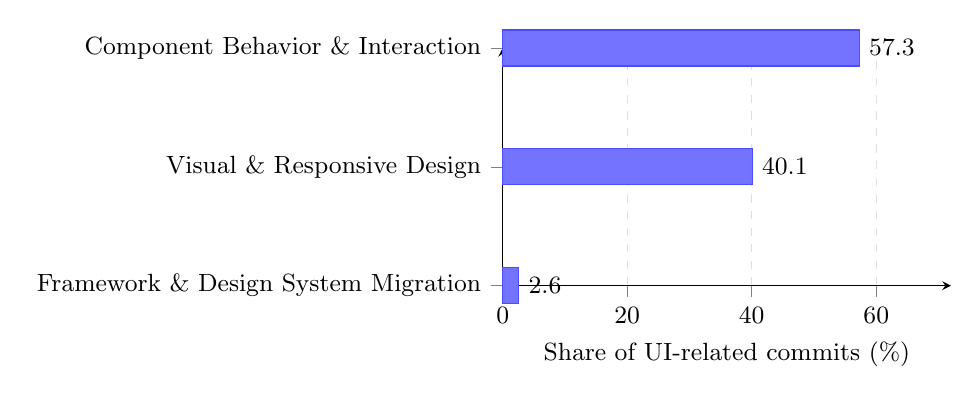
\begin{tikzpicture}
\begin{axis}[uidistbar,
    symbolic y coords={Framework \& Design System Migration,
                       Visual \& Responsive Design,
                       Component Behavior \& Interaction}]
\addplot[fill=blue!55, draw=blue!70] coordinates {
    (57.3,Component Behavior \& Interaction)
    (40.1,Visual \& Responsive Design)
    (2.6,Framework \& Design System Migration)};
\end{axis}
\end{tikzpicture}
\caption{Distribution of Modernization \emph{Aspects} across all UI-related
commits in the mined pool (LLM-classified).}
\label{fig:aspects-full}
\end{figure}

\begin{figure}[htbp]
\centering
\begin{tikzpicture}
\begin{axis}[uidistbar,
    symbolic y coords={Accessibility Compliance (A11y),
                       Architectural Layout Drift \& Preferences,
                       Usability Friction \& Component Degradation}]
\addplot[fill=teal!60, draw=teal!80] coordinates {
    (60.6,Usability Friction \& Component Degradation)
    (36.2,Architectural Layout Drift \& Preferences)
    (2.6,Accessibility Compliance (A11y))};
\end{axis}
\end{tikzpicture}
\caption{Distribution of Modernization \emph{Causes} across all UI-related
commits in the mined pool (LLM-classified).}
\label{fig:causes-full}
\end{figure}

\paragraph{How each commit was assigned an Aspect and a Cause.}
Each UI-related commit was assigned exactly one \emph{Aspect} (\emph{what}
changed in the interface) and one \emph{Cause} (\emph{why} the change was
made), inferred from the commit message together with the repository
context. The \emph{Aspect} captures the structural nature of the change and
maps one-to-one onto the modernization spectrum
(Section~\ref{sec:spectrum}). A commit was labelled \textbf{Component
Behavior and Interaction} (Up-Level) when it altered how a component reacts
to input or state --- e.g., hover, focus, or disabled feedback, animations
and transitions, navigation, pagination or scrolling, input handling, or the
repair of a broken, frozen, or flickering interaction. It was labelled
\textbf{Visual and Responsive Design} (Intermediate-Level) when it changed
only the appearance of existing components without altering their behavior
--- color, spacing, typography, theming, light/dark mode, alignment, icons,
or responsive breakpoints. It was labelled \textbf{Framework and Design
System Migration} (Down-Level) when it adopted, replaced, or upgraded a UI
library or design system, introduced or propagated design tokens, or moved
components onto a shared component library.

The \emph{Cause} captures the human-centric trigger behind the change,
following the three categories of Section~\ref{sec:method}. A commit was
assigned \textbf{Accessibility Compliance} when it explicitly targeted an
accessibility barrier --- ARIA attributes, colour-contrast, screen-reader
support, keyboard operability, or touch-target sizing. It was assigned
\textbf{Architectural Layout Drift and Preferences} when it re-aligned
elements to a design guideline, repositioned or reconfigured interface
elements, adjusted spacing or theme configuration, or added a user
preference or toggle. It was assigned \textbf{Usability Friction and
Component Degradation} when it removed visual clutter or resolved an
operational defect degrading the experience --- flicker, overflow, a stuck
loader, a rendering glitch, or a frozen interaction. When a commit carried
signals for more than one category (for instance, a dark-mode contrast fix
that is both an accessibility and a visual change), the \emph{dominant}
change described in the message --- the primary problem the commit set out
to solve --- determined the label, so that every commit contributes to a
single Aspect and a single Cause and the two distributions are directly
comparable.
